\chapter{Recommender Systems and Social Networks}
\label{c:recommendersystemsandsocialnetworks} This chapter is dedicated to the introduction of the relevant theoretical concepts that need to be understood in order to properly comprehend social recommender systems. It is arranged in three sections: The first section gives an overview over recommender systems' history, application areas and theoretical concepts. It also defines a formal framework for recommender algorithms and presents the different algorithmic approaches used in the experiments (chapter \ref{c:experiments}). The second section is devoted to social networks and their properties. Understanding social networks and their properties is important for the incorporation of information into recommender systems and also for the generation of artificial social networks (chapter \ref{c:artificialdatageneration}). The third section then combines the two fields by introducing recommendation algorithms that incorporate social network information, thus creating social recommender systems.

\section{Recommender Systems}
\label{st:recommendersystems} People face the challenge of making decisions and weighing different options every day. Often they take into consideration not only their own opinion and knowledge, but also the advice and recommendations of others. But these methods have their limits. A user might for example never hear about a good book that he would really like, if none of his friends knows that book. And often the almost infinite number of alternatives (e.g. what movie to watch or what music to listen to) makes it impossible to properly evaluate all options and find the best one. This is where a computer-based system can outperform human recommendations. Recommender systems are tools that try to predict the valuation users have for different items. They aim at helping the user in his decision-making processes, like what items to buy, what movies to watch or what music to listen to. Advantages over human recommendations include the much larger set of recommenders (even people who do not know a user personally might contribute some valuable information), the more systematical inclusion of a user's history and his already expressed preferences and the possibility to computationally deal with a much larger amount of alternatives. The possible application space of recommender systems is endless and there exist real-world examples in many different areas like books, restaurants, financial services \cite{Felfernig_2007} or even persons (online dating).

There are a lot of factors that determine the goodness and the practical success of recommender systems. Different application areas demand different abilities. In some areas, speed might be the crucial factor, in others transparency might be critical (users want to know how the recommendations are made), or it might be the case that users want a very broad range of new items recommended instead of only very similar ones. In reality, recommender systems are often used in commercial settings and the design of a particular recommender system should be highly dependent on the environment where it will be used. It is important to carefully evaluate the requirements posed by the environment and build the recommender system according to those requirements.
\newline

As a consequence of the various conditions and surroundings recommender systems operate in, there exist many different approaches and recommendation techniques. \cite{Ricci_2011} give a good overview over existing methods and algorithms. Here, two of the most popular approaches are described, while the focus of the experiments lies explicitly on the collaborative filtering approach.

\subsection{Content-Based Filtering}
\label{sst:contentbasedfiltering} Content-based filtering looks at the similarity between different items. Based on the attributes and characteristics of items a user has rated in the past, the system will recommend new items with similar characteristics to the user. If someone has watched a lot of action movies with Sylvester Stallone (and given them a good rating), it is likely that movies starring Sylvester Stallone or movies belonging to the action genre will be recommended to this person. Whereas in movies one often has to make appropriate categorizations manually, this process can be automated with text-based content (like books or webpages). Text can be scanned for frequently used keywords and recommendations can be made based on keyword frequency.

\subsubsection{Challenges}
\label{ssst:challenges} There are numerous challenges to this approach. One that was already mentioned before is the categorization of items. Where content is not text-based, it is hard to automatically extract information about the content, especially in movie or music domains. Another problem is the new-user problem: It is hard to provide accurate recommendations for new users who have only rated very few items so far, since there is not much information about their preferences. Furthermore, there exists also the danger of over-specialization, which means that the user from the Sylvester Stallone example might never be recommended a comedy movie if he has not watched one yet, even though he might actually like it.

\subsection{Collaborative Filtering}
\label{sst:collaborativefiltering} The method of collaborative filtering does not use any information about items' characteristics in order to make predictions. Instead it takes into account the rating history of all users. This new approach already addresses one of the big challenges of content-based methods, that is the high categorization-cost. The new-user problem still exists, but is less severe.

In user-based collaborative filtering, the idea is to find users with similar rating behaviour and predict ratings for an item based on these similar users' ratings for this item. Item-based collaborative filtering tries to find items that have been rated similarly across all users and then makes a prediction for an item based on the user's ratings for similar items.

\subsubsection{Challenges}
\label{ssst:challengescf} As already mentioned, some of the main challenges of content-based filtering can be avoided with this approach, however there occur other, new challenges. The main difficulty with collaborative filtering can be the extremely high computational cost. Calculating all user-similarities can be a serious issue, especially in domains with thousands of users and possibly millions of items.

\subsection{Formal Framework}
\label{sst:formalframework} To mathematically describe the different algorithms and metrics that are used in the experiments, a formal framework is introduced here. Let $U = \{1,...,u\}$ denote the set of users and let $G = \{1,...,g\}$ denote the set of items. Let $r_i(j)$ denote the actual rating of user $i \in U$ for item $j \in G$. The ultimate task for every recommender system is to find a good estimate $\hat{r}_i(j)$ for an item $j$ that user $i$ has not rated yet. The closer $\hat{r}_i(j)$ is to the user's actual rating $r_i(j)$ (which exists even if the user has not explicitly rated the item yet; it should be seen as the actual valuation of the user for that item), the more accurate the recommendation is.

As mentioned above, there exist many aspects that contribute to the quality of a recommender system and the performance might be highly dependent on the environment the system operates in. Nevertheless, accuracy is considered to be the most important metric to measure the performance of a recommender system. One common measure to express the accuracy is the \textit{root-mean-square error} (RMSE). For a series of $n$ predictions $\hat{r}_n$ and actual ratings $r_n$, it is defined as follows:

\begin{equation}
RMSE = \sqrt{\frac{1}{n} \sum_{i=1}^{n}(r_n - \hat{r}_n)^2}
\label{eq:rmse}
\end{equation}

\subsubsection{Similarity Measures}
\label{ssst:similaritymeasures} User-based collaborative filtering tries to find users that are similar to a particular user. The assumption is that similar users will be good predictors for the estimation of $\hat{r}_i(j)$. The first step is thus to find a measure of similarity between two users. There exist different measures, of which two commonly used ones will be presented.
\newline

\textbf{Pearson Correlation Coefficient} The Pearson correlation coefficient measures the similarity between two users $i$ and $i'$. Let $\bar{r}_i$ denote the average rating over all items user $i$ has rated so far. $G_{ii'}$ ist the set of items both users have already rated. Then the Pearson correlation coefficient is calculated as follows:

\begin{equation}
sim(i,i') = \frac{\sum_{j \in G_{ii'}}{(r_i(j)-\bar{r}_i)(r_{i'}(j)-\bar{r}_{i'})}}{\sqrt{\sum_{j \in G_{ii'}}{(r_i(j)-\bar{r}_i)^2}}\sqrt{\sum_{j \in G_{ii'}}{(r_{i'}(j)-\bar{r}_{i'})^2}}}
\label{eq:pearson}
\end{equation}

The pearson correlation coefficient results in a similarity value between $-1$ and $+1$.
\newline

\textbf{Cosine Similarity Coefficient} A second similarity measure that is widely used to calculate how similar two users are is the cosine similarity. The cosine similarity calculates the similarity of orientation of two vectors. The two vectors $x_i$ and $x_{i'}$ in this case are the rating vectors of users $i$ and $i'$ respectively, containing all ratings $r_{i}(j)$ and $r_{i'}(j)$ respectively of the items in set $G_{ii'}$. The cosine similarity is then calculated as follows:

\begin{equation}
sim(i,i') = \frac{\sum_{j \in G_{ii'}}{r_{i}(j)\cdot r_{i'}(j)}}{\sqrt{\sum_{j \in G_{ii'}}{{r_{i}^2}(j)}}\sqrt{\sum_{j \in G_{ii'}}{{r_{i'}^2}(j)}}}
\label{eq:cosine}
\end{equation}

The similarities calculated with equation \eqref{eq:cosine} also lie in the range from $-1$ to $+1$.
\newline

Once all similarities $sim(i,i')$ for a user $i$ are calculated, the other users can be sorted by their similarity to user $i$. It makes sense to only consider the most similar users for the prediction of $\hat{r}_i(j)$, since their ratings correlate the most with user $i$'s ratings. The next step is thus to choose an appropriate subset of all users $i'$, which is called the \textit{neighbourhood} $N$ of a user. The size of this neighbourhood can be determined in different ways, it can either be a certain number (e.g. 50) or it can be determined through applying a threshold on the similarities (e.g. only include users with similarity greater than 0.5).

\subsubsection{Prediction Measures}
\label{ssst:predictionmeasures} Once this neighbourhood set is determined, there exist different ways to compute the estimated rating $\hat{r}_i(j)$. We consider two approaches and a third one that combines the first two.
\newline

\textbf{Weighted Sum} The weighted sum aggregation takes into account that more similar users should have a bigger influence on the prediction than less similar ones. To predict rating $\hat{r}_i(j)$, the rating for item $j$ of each user $i'$ in the determined neighbourhood $N$ is weighted with $sim(i,i')$:

\begin{equation}
\hat{r}_i(j) = \frac{\sum_{i' \in N}{sim(i,i')\cdot r_{i'}(j)}}{\sum_{i' \in N}{sim(i,i')}}
\label{eq:weightedsum}
\end{equation}
\newline

\textbf{Adjusted Sum} A problem that the weighted sum aggregation does not take into account is that users might interpret the rating scale differently. Some users might generally give lower ratings than others. To account for this, the adjusted sum prediction uses the average rating $\bar{r}_{i'}$ of each user $i'$.

\begin{equation}
\hat{r}_i(j) = \bar{r}_i + \frac{\sum_{i' \in N}{r_{i'}(j)\cdot \bar{r}_{i'}}}{\mid N\mid}
\label{eq:adjustedsum}
\end{equation}
\newline

\textbf{Adjusted Weighted Sum} The adjusted weighted sum combines both aspects; it weighs the users' ratings by their similarity and it adjusts the ratings with the average ratings:

\begin{equation}
\hat{r}_i(j) =  \bar{r}_i + \frac{\sum_{i' \in N}{sim(i,i')\cdot (r_{i'}(j) - \bar{r}_{i'})}}{\sum_{i' \in N}{sim(i,i')}}
\label{eq:adjustedweightedsum}
\end{equation}

Note that in all three approaches the sum is over all users in neighbourhood $N$. One has to take into account the fact that it is not certain that all users in $N$ have already rated item $j$. In fact, the sparser the rating matrix, the higher the probability that there are users who have not rated item $j$ and are therefore left out of the prediction calculation. The actual set of neighbours that influence $\hat{r}_i(j)$ can therefore be much smaller than $\lvert N \rvert$.

\subsection{Related work}
\label{sst:rsrelatedwork} There is a vast variety of studies and papers that give a survey on the topic of recommender systems. \cite{Ricci_2011} give a good overview over existing approaches to recommender systems and explain in detail different properties of recommender algorithms. A recommender algorithm can be evaluated and compared to others with respect to these properties. By far the most used property to assess the quality of a recommender algorithm is its prediction accuracy. Since recommender algorithms aim at providing recommendations to users, it is safe to assume that users prefer algorithms that have a high prediction accuracy, that is they predict ratings that are close to the actual rating of a user.

\cite{Adomavicius_2005} describe the state-of-the-art of recommender algorithms and give theoretical background on content-based, collaborative filtering and hybrid approaches. They further suggest possible extensions to enhance these algorithms.

\section{Social Networks}
\label{s:socialnetworks} Social networks are structures that have existed for a very long time. It is even safe to say that people would not be able to live by themselves, without any social connections. There exist many kinds of social ties between people, including friendships, family, or also work-related relationships. A social network is basically made up of two components; the social actors (which often are people, but could also be organizations or other social entities) and the ties between those actors.

Whereas in the past social network structures were often implicitly present, but hard to explicitly capture and analyze, the rise of the internet and the effects of globalization are responsible for the appearance of online social networks like Facebook or Twitter. These networks often are a good reflection of real social networks, with the big advantage that they can be empirically studied and analyzed.

\subsection{Formal Framework}
\label{sst:formalframeworkgraphs} Social networks can be mathematically represented by graphs. A graph consists of a set of nodes $v \in N$ and a set of edges $e \in E$ which are dyadic links between two nodes. Graphs are often drawn with nodes as little circles and edges as connecting lines between the circles. The edges can either be undirected, meaning that the relationship is bi-directional, or they can be directed (drawn as arrows instead of lines) meaning that the relation goes only in one direction.

\begin{figure}[!ht]
\centering
\begin{minipage}[b]{5 cm}
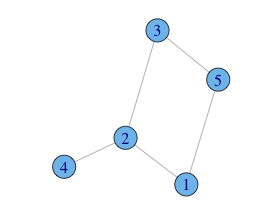
\includegraphics[width=150px]{./2-recommendersystemssocialnetworks/figures/SampleGraph.png}
\label{f:simplegraph}
\end{minipage}
\begin{minipage}[b]{5 cm}
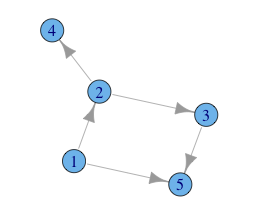
\includegraphics[width=150px]{./2-recommendersystemssocialnetworks/figures/SampleGraph2.png}
\label{f:simplegraph}
\end{minipage}
\caption[An undirected and a directed graph, each with 5 nodes and 5 edges.]
{An undirected and a directed graph, each with 5 nodes and 5 edges.}
\end{figure}

In the space of online social networks, a Twitter graph would be a directed graph because you can follow a person without this person following you. The Facebook social network would be represented as an undirected graph, since friendships are always bi-directional. For this thesis, we will only consider two-way friendships and thus we will always work with undirected graphs. Edges can also be weighted, with the weight of an edge indicating the strength of the tie between two nodes. This aspect is also not of importance in the networks studied in this thesis and therefore edges will not be weighted, or in other words will all have the same weight 1.

\subsection{Graph Properties}
\label{sst:graphproperties} Once an existing social network is transformed into its mathematical representation, a graph, we can analyze different properties of this graph in order to find out more about the structure of the network. Different properties of a graph are presented and also properties that are characteristic for real-world social networks will be explained. This will play a big role in the graph generation section, where the task is to generate networks with realistic social network properties.
\newline

\textbf{Degree} The degree of a node is the number of edges adjacent to it. In a social network where edges represent friendships the degree is the number of friends someone has.
\newline

\textbf{Distance} The distance between two nodes is the number of edges of the shortest path between those two nodes. A path is a sequence of edges that connect a sequence of nodes, and the shortest path between two nodes is the path that connects those two nodes through the least number of edges (note: there can be multiple shortest paths between two nodes). In a social network where edges represent friendships between people, all your direct friends would have distance 1 from you, and friends of your friends would have distance 2.
\newline

\textbf{Average Path Length} The average path length is the average length of the shortest paths of all possible node pairs. It is an indicator of how well information or data can be transported through a network. A shorter average path length means that information will spread across the network faster.
\newline

\textbf{Global Clustering Coefficient/Transitivity} The clustering coefficient of a graph (also called transitivity) measures the tendence of nodes to cluster together and form cliques. A clique is a set of nodes where every node is connected to every other node. The clustering coefficient is defined as $\frac{3\:\times\:number\:of\:triangles}{number\:of\:connected\:triples}$, where a triangle is 3 nodes all connected with each other (a clique of size 3) and a connected triple is 3 nodes where at least one node is connected with both other nodes.

There also exists a local clustering coefficient which measures how close one node's neighbours are to being a clique.
\newline

\textbf{Centrality} The concept of centrality is a way to measure the importance of a node within a network. In social networks, it can be used to find influential users, e.g. users that have a big influence on others' opinion and taste. Centrality measures are functions that provide values for every node, which can then be sorted to produce a ranking from the most to the least central node.
\newline

\textbf{Betweenness Centrality} Betweenness centrality is a measure that gives every node a value which indicates its importance within the network. The number each node $v$ receives is equal to the number of shortest paths that pass through $v$.

\begin{equation}
g(v) = \sum_{s \neq v \neq t} \frac{\sigma_{st}(v)}{\sigma_{st}}
\label{eq:betweennesscentrality}
\end{equation}

$\sigma_{st}$ stands for the total number of shortest paths from node $s$ to node $t$, and $\sigma_{st}(v)$ is the number of those shortest paths that go through $v$.

Given this definition, the betweenness score in large networks can be very high. To receive normalized scores $g \in [0,1]$, one can divide $g$ by the total number of node pairs not including $v$.

\subsection{Social Network Characteristics}
\label{sst:socialnetworkcharacteristics} There exist many different social networks. There are social networks like Facebook where friends share content and keep in touch, scientific collaboration networks or also social ties on music streaming sites like last.fm \cite{Lastfm}. Of course the sizes and specific structures of those networks might vary, depending on the application area. But still there exist characteristics that most social networks seem to share and that makes it possible to distinguish them from other classes of networks. \cite{Newman_2003} and \cite{Zaidi_2012} establish three main characteristics of social networks:
\newline

\textbf{Scale-free Network} Social networks often are scale-free networks. A scale-free network has a degree distribution that approximately follows a power law. A power law is a function of the form $f(x) = \alpha x^{-\gamma}$. The fraction of nodes $P(k)$ with degree $k$ is then $P(k) \sim k^{-\gamma}$, with $\gamma$ often found to be in between 2 and 3.

The reason this node degree distribution is often found in social networks is that most people tend to know only few other people, while very few people (e.g. celebrities) have considerably more social connections. The process of \textit{preferential attachment} (people who already have much connections over time tend to make even more connections than people with only few connections) accounts for this distribution. The development of this structure often comes very naturally, e.g. in a mathematic collaboration network where a mathematician has already contributed to many studies and is therefore quite popular, he is more likely to collaborate with even more people than other, not very popular mathematicians.
\newline

\textbf{Small-world Network} Social networks also tend to reveal the small-world phenomenon. This phenomenon was first studied by \cite{Milgram_1967} and \cite{Travers_1969} who conducted an experiment where people all over the United States were randomly chosen as ``starters'' that had the task to forward a message to a designated ``target'' person as fast as possible, with the only rule that they were only allowed to send the letter to someone they knew on a first-name basis. A surprisingly high number of messages reached the target, and the astonishingly low median of steps from the starter to the target was 6. This experiment has been the trigger of more research and has led to the term small-world network. A small-world network is a network with a low average path length (the average path length grows logarithmically to the number of nodes).
\newline

\textbf{Community Structure} The third characteristic of social networks is that they tend to consist of communities. Communities are parts of the network with densely connected nodes, while connections between different communities are scarcer. There is no mathematical definition for community structure, which makes it often hard to algorithmically find in networks. However, there exist many approaches to this problem, of which the most important ones are described in section \ref{sst:communityalgorithms}. It is also easy to understand the presence of communities in social networks, \textit{triadic closure} \cite{Easley_2010} is one of the main reasons (two people who have a friend in common are more likely to get to know each other than two random people are) for the formation of communities.

\subsection{Related Work}
\label{sst:snrelatedwork} \cite{Easley_2010} give a broad introduction into many of the network related topics discussed in this thesis. \cite{Newman_2003} show why and how social networks differ from other types of networks.

\section{Social Recommender Systems}
\label{st:socialrecommendersystems} Conventional CF does not take into account any social relations that might exist between users to form an appropriate neighbourhood. The neighbourhood is selected solely by a similarity measure that compares users' ratings. This is done because it is assumed that similar users are the best predictors. But a user might give more weight to a friend he personally knows than to a complete stranger, and moreover a friend might know more about the user's preferences and he might also have a similar taste. Often people hang out with people sharing common interests and having similar tastes (e.g. music taste, travelling, political interest etc.). This gives rise to the combination of CF and social networks - social recommender systems. Although there exist different approaches, here we will focus on social collaborative filtering (social CF), which will be introduced in more detail.

\subsection{Social Collaborative Filtering}
\label{sst:socialcf} Social CF differs from CF only in the way the neighbourhood set $N$ is chosen. Instead of taking into account the most similar users, one can take as neighbourhood set a user's direct friends in the network. Since the set of direct friends can be quite small, it could also be advisable to take into account the friends of a user's friends. This can be done for bigger distances, although this process of traversing the friend graph quickly gets very time-consuming and also does not make that much sense in terms of social contacts. With distance 2 or 3, it is already likely that there are many people in the neighbourhood set that you do not know at all, and with a distance of more than 3 it is almost certain that most people in the set will have almost no relation to you. In addition to this, one can also apply a similarity threshold on the neighbourhood set in order to filter out friends or friends of friends that might not be similar to a user.

All other steps stay the same as in conventional CF; the similarity calculation between all users as well as the prediction calculation are performed in the same way.